\chapter{Benchmarks en Experimenten}
% \chaptermark{Een kortere titel voor de paginahoofding (verschillend van titel in TOC)}

\todo[inline,caption={}]{Terminologie?

\begin{itemize}
	\item Object (geretourneerde gegevens.) <-> OID's (kunnen subtakken zijn van meerdere OID's)
	\item SNMP Data Retriever
	\item Relevante OID's/objecten/gegevens
\end{itemize}

}

\section{Kleinschalige benchmarks en experimenten}

\subsection{Testopstelling}

\todo[inline]{Enerzijds de Virtual Box opstelling. Anderzijds heb je ook de iMinds switchen.}


\subsection{Profiling van de SNMP Data Retriever}

\todo[inline]{Cleanup. Aanvullen na afwerken. \\
Is het een probleem dat functies en methoden door elkaar gebruikt worden?}
In deze sectie gaan we de SNMP Data Retriever van NetworkMining onder de loep nemen met de ingebouwde profiler van Visual Studio.
Een profiler zal ons enkele belangrijke inzichten verschaffen over wat er achter de schermen gebeurt bij het uitvoeren van de retriever.
Specifiek:

\begin{itemize}
	\item Hoe lang bepaalde stukken code er over doen
	\item Hoe vaak bepaalde stukken code uitgevoerd worden (zogenaamde hot code/paths)
	\item Problematische stukken code detecteren die er veel langer over doet dan we verwachten
	\item En bijgevolg welke stukken het meeste potentieel bieden om te optimaliseren
\end{itemize}

\subsubsection{Gebruik van de profiler in Visual Studio 2013}

De profiler in Visual Studio 2013 is erg makkelijk te gebruiken.
Om te beginnen open je je project en klik je op \emph{Analyze} in de werkbalk en kies je voor \emph{Performance and Diagnostics}.
Als alternatief kun je ook van de ALT+F2 sneltoets gebruik maken.\todo{Koppelteken}
Als \emph{Target} staat standaard het huidige project geselecteerd.
Onder \emph{Available Tools} zou normaal ook de \emph{Performance Wizard} moeten geselecteerd zijn.
Zoals de beschrijving al verklapt houdt dit onder andere het meten van CPU- en RAM-gebruik in.
Als je op \emph{Start} klikt krijg je de \emph{Performance Wizard} te zien (\figurenamesentence{} \ref{performance-wizard}).
Hier moet je kiezen van welke profilingmethode je wenst gebruik te maken.
Wij kiezen voor de eerste: \emph{CPU Sampling}.
De rest van de stappen staan standaard goed dus mag je meteen op \emph{Finish} klikken.

\begin{figure}[]
	\centering
	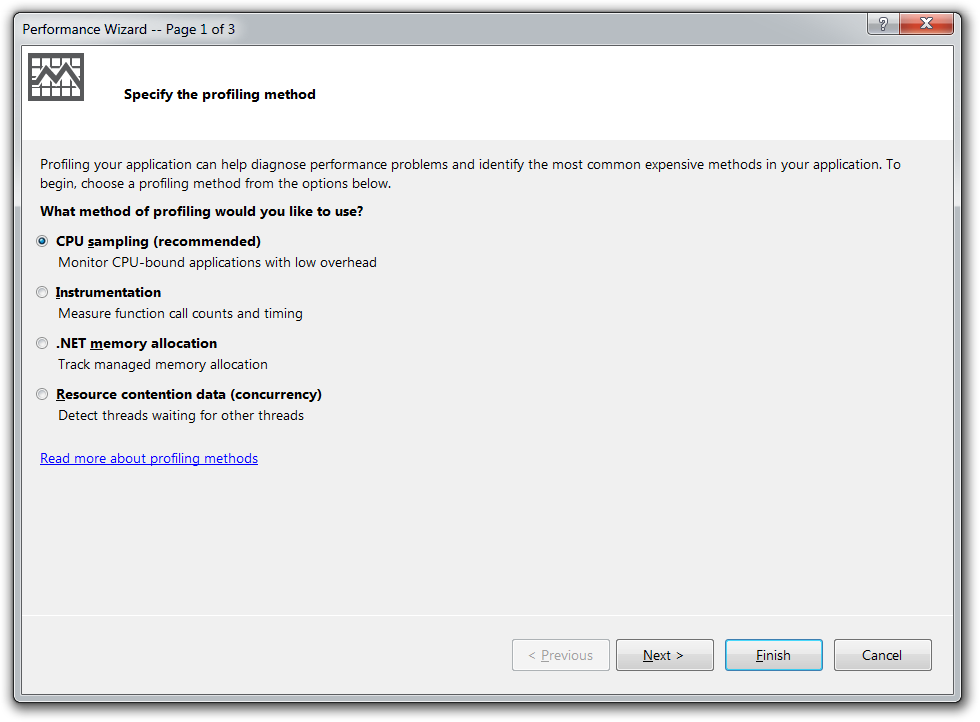
\includegraphics[scale=0.50]{figures/profiler/performance-wizard}
	\caption{De Performance Wizard}
	\label{performance-wizard}
\end{figure}

Wanner het programma klaar is met uitvoeren worden de resultaten geanalyseerd.
Als dat klaar is krijg je een algemeen overzicht van de resultaten. \todo{gedaan?}
Eerst en vooral zie je een grafiek met het CPU-gebruik doorheen de uitvoeringstijd van de applicatie.
Daaronder zie je de \emph{Hot Paths}, dat zijn de functies die verantwoordelijk zijn voor het grootste deel van de uitvoeringstijd.
Waar wij in geïnteresseerd zijn is hieraan gerelateerd: de \emph{Call Tree View}.
Die geeft je een boomstructuur van functies die elkaar oproepen en enkele belangrijke statistieken:
hoeveel keer een functie werd opgeroepen en hoeveel tijd de functie gemiddeld nodig had om uit te voeren,
dit zowel procentueel (ten opzichte van de totale uitvoeringstijd) als in absolute tijd.

De call tree van de SNMP Data Retriever kun je zien in \figurenamesentence{} \ref{call-tree}.
Hierbij werd de \emph{Main} functie opengeklapt.\todo{Koppelteken}
Je kunt functies verder open klappen om te zien welke andere functies worden opgeroepen en hun aandeel in de uitvoeringstijd analyseren.
Dit kan verder gaan tot je atomaire functies krijgt die geen andere functies meer oproepen.

In de call tree zie je naast de functienaam een aantal verschillende kolommen. Hieronder volgt de lijst van de kolommen en hun betekenis.

\begin{itemize}
	\item \textbf{Number of calls:}
		dit spreekt vrij voor zichzelf. Dit is het aantal keren dat een functie opgeroepen werd.
	\item \textbf{Elapsed Inclusive Time \%:}
		dit is het percentage van de uitvoeringstijd dat werd gespendeerd in deze functie en zijn kinderen.
	\item \textbf{Elapsed Exclusive Time \%:}
		dit is het percentage van de uitvoeringstijd dat uitsluitend in deze functie werd gespendeerd, dus \emph{exclusief} zijn kinderen.
	\item \textbf{Avg Elapsed Inclusive Time:}
		dit is de gemiddelde uitvoeringstijd in milliseconden van deze functie en zijn kinderen.
	\item \textbf{Avg Elapsed Exclusive Time:}
		dit is de gemiddelde uitvoeringstijd in milliseconden van uitsluitend deze functie, dus weer \emph{exclusief} zijn kinderen.
		\todo{Check of er geen pagebreak is op de individuele items.}
\end{itemize}

\begin{figure}[h]
	\centering
	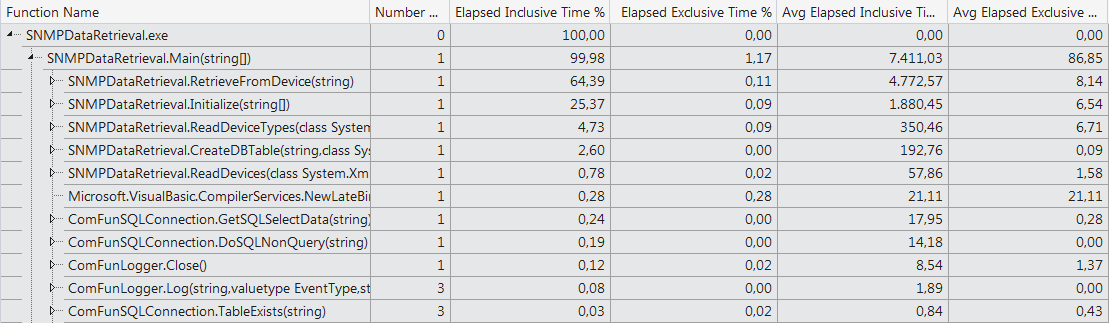
\includegraphics[scale=0.50]{figures/profiler/call-tree}
	\caption[De Call Tree]{De Call Tree. De kolommen van links naar rechts:
		\emph{Function Name},
		\emph{Elapsed Inclusive Time \%},
		\emph{Elapsed Exclusive Time \%},
		\emph{Avg Elapsed Inclusive Time},
		\emph{Avg Elapsed Exclusive Time}.}
	\label{call-tree}
\end{figure}

\subsubsection{De resultaten}

Voor het wegschrijven van de resultaten van de SNMP Data Retriever installeren we een lokale databank.
\todo{Vertellen we waarom?}
De retriever verwacht een MySQL databank, maar wij kiezen voor een MariaDB-installatie.
Omdat MariaDB een drop-in vervanging is voor MySQL is dat echter geen probleem.
Op het moment van installatie was de laatste stabiele versie 5.5.33a.

We doen een walk van 2 \glspl{oid} op een enkele productieswitch. Dit zal ons 443 objecten opleveren,
waarvan 441 die voor ons relevant zijn. Volgens de profiler doet de retriever daar ongeveer 7,4 seconden over.
De call tree van de retriever hebben we voor de leesbaarheid in een tabel gegoten (zie \tablenamesentence{} \ref{call-tree-main}).
De functies met een extreem kleine uitvoeringstijd (minder dan 0,01\%) hebben we achterwege gelaten.
De kolommen die je ziet zijn de functie, het aantal oproepen, de \emph{inclusieve} tijd als percentage van de totale uitvoeringstijd en
de gemiddelde \emph{inclusieve} tijd in milliseconden.

% Loglevel 2
\begin{table}[h]
	\centering
	\begin{tabular}{@{}lrrr@{}}
		\toprule
		Functie                                                  & Calls & Tijd (\%) & Tijd (ms) \\ \midrule
		SNMPDataRetrieval.RetrieveFromDevice                     & 1     & 64,39     & 4.772,57  \\
		SNMPDataRetrieval.Initialize                             & 1     & 25,37     & 1.880,45  \\
		SNMPDataRetrieval.ReadDeviceTypes                        & 1     & 4,73      & 350,46    \\
		SNMPDataRetrieval.CreateDBTable                          & 1     & 2,60      & 192,76    \\
		SNMPDataRetrieval.ReadDevices                            & 1     & 0,78      & 57,86     \\
		Microsoft.VisualBasic.CompilerServices.NewLateBinding.L… & 1     & 0,28      & 21,11     \\
		ComFunSQLConnection.GetSQLSelectData                     & 1     & 0,24      & 17,95     \\
		ComFunSQLConnection.DoSQLNonQuery                        & 1     & 0,19      & 14,18     \\
		ComFunLogger.Close                                       & 1     & 0,12      & 8,54      \\
		ComFunLogger.Log                                         & 3     & 0,08      & 1,89      \\
		ComFunSQLConnection.TableExists                          & 3     & 0,03      & 0,84      \\ \bottomrule
	\end{tabular}
	\caption{De call tree van de Main methode} %TODO: Koppelteken
	\label{call-tree-main}
\end{table}

We beginnen met de functie die het meeste tijd in beslag neemt: de \emph{RetrieveFromDevice} functie. \todo{Koppelteken}


\todo[inline]{Herschrijf begin van stuk over logging framework.}
Het eerste wat er ons opvalt als we de call tree bekijken is dat de \emph{Initialize} methode 25\% van de
uitvoeringstijd voor zijn rekening neemt.
Rijst de vraag wat deze functie juist doet dat ze zoveel tijd nodig heeft.

We klappen de Initialize methode open om de boosdoeners te zoeken.
De functies van de Initialize methode vind je terug in \tablenamesentence{} \ref{call-tree-initialize}.
We zien twee oproepen naar een \emph{Log} methode die er gemiddeld bijna een seconde over doet \emph{per oproep}! \todo{Koppelteken}

\begin{table}[h]
	\centering
	\begin{tabular}{@{}lrrr@{}}
		\toprule
		Functie                                                   & Calls & Tijd (\%) & Tijd (ms) \\ \midrule
		ComFunLogger.Log                                          & 2     & 20,97     & 777,30    \\
		ComFunSQLConnection..ctor                                 & 1     & 3,51      & 259,97    \\
		ComFunLogger.set\_LogFile                                 & 1     & 0,19      & 13,87     \\
		System.Configuration.ConfigurationManager.get\_AppSettin… & 12    & 0,16      & 0,99      \\
		Microsoft.VisualBasic.CompilerServices.Conversions.ToIn…  & 2     & 0,15      & 5,58      \\
		ComFunLogger.Log                                          & 4     & 0,13      & 2,41      \\
		ComFunLogger.Log                                          & 3     & 0,06      & 1,59      \\
		ComFunLogger.Log                                          & 2     & 0,05      & 1,87      \\
		ComFun.NetworkMiningCopyRightStatement                    & 1     & 0,03      & 2,03      \\
		ComFunLogger..ctor                                        & 1     & 0,01      & 1,10      \\ \bottomrule
	\end{tabular}
	\caption{De call tree van de Initialize methode}
	\label{call-tree-initialize}
\end{table}

De \emph{ComFunLogger} is een stuk code die gebruikt wordt om te loggen naar een tekstbestand.
De naam komt van het feit dat ze een gemeenschappelijk stuk code is die over meerdere projecten kan
gebruikt worden: \emph{common functions}, of \emph{ComFun} voor kort.
Maar een functie die loggegevens wegschrijft naar een bestand hoort niet zo lang te duren.
I/O operaties zijn kostelijk, maar niet \emph{zo} kostelijk. \todo{Koppelteken}
Als we de functie helemaal openklappen in \figurenamesentence{} \ref{call-tree-performancecounter} vinden we de echte dader:
een constructor van \emph{System.Diagnostics.PerformanceCounter}.
Een performance counter wordt gebruikt voor het monitoren van systeemcomponenten zoals
processoren, geheugen en netwerk I/O. Als je ze gebruikt in je applicatie kunnen ze je \todo{Koppelteken}
informatie geven over de performantie van je programma.\cite{performance-counters-intro}
De ComFunLogger gebruikt ze om het geheugengebruik te meten en weg te schrijven in de logbestanden.

\begin{figure}[h]
	\centering
	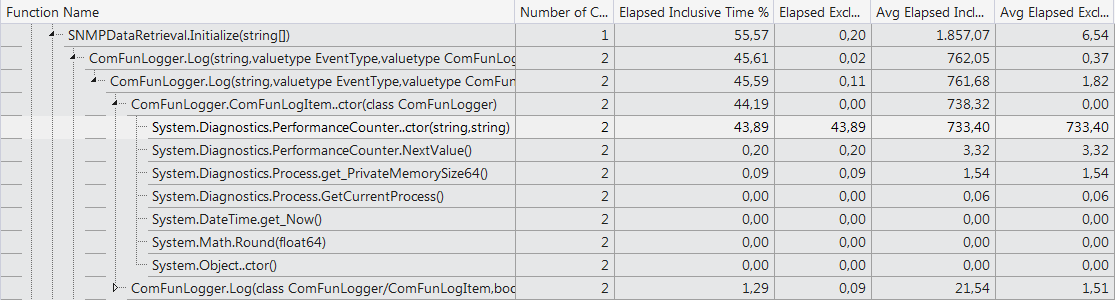
\includegraphics[scale=0.50]{figures/profiler/call-tree-performancecounter}
	\caption{De call tree van de Log methode}
	\label{call-tree-performancecounter}
\end{figure}

\todo[inline]{Herlees mij.}

Als oplossing werd ervoor gekozen om een alternatieve \emph{logging framework} te gebruiken.
Dit lijkt een drastische maatregel (en dat is het ook), maar daar zijn goede redenen voor.
Er zijn een heleboel gratis en open-source logging frameworks die reeds hun nut en kunnen bewezen hebben.
Zij zijn \emph{tried and true} oplossingen voor een algemeen probleem. \todo{Het zijn...}
Het is dus ook in de beste interesse voor een bedrijf om hiervoor te kiezen. \todo{Correcte zin?}
Financiëel is het een goede oplossing want de software is al ontwikkeld en is bewezen dat ze werkt.
Dit spaart tijd en geld uit voor de ontwikkeling van een eigen oplossing.
De software is gratis in gebruik dus er zijn geen licentiekosten aan verbonden.
Er zijn ook geen of lage onderhoudskosten. De software wordt al ingezet in zeer diverse omgevingen dus is al zeer uitgebreid.
De kans dat de software een bepaalde functionaliteit mist is dus klein.
En als er iets moet toegevoegd worden beschik je ook over de broncode.

Ook vanuit technisch opzicht is het een goede keuze.
Zoals gezegd heeft de software al zijn nut bewezen in diverse omgevingen.
In het specifieke geval van de ComFunLogger biedt een \emph{third party} oplossing ook een heleboel
extra flexibiliteit en features. Zo kan je loggen naar meerdere outputs en zijn er meerdere mogelijke outputs beschikbaar.
Je kunt bijvoorbeeld loggen naar tekstbestanden, consolevensters, databanken, enzovoort.

De twee belangrijkste redenen echter zijn het feit dat ze ontwikkeld zijn om een zo klein mogelijke performantieimpact te hebben en
dat de implementatie zeer simpel is.
Zo was het veel sneller om een ander logging framework te gebruiken dan om bekend te raken met de bestaande loggingcode en die te optimaliseren.

De keuze is uiteindelijk gevallen op Apache log4net en is gebaseerd op waarschijnlijk het bekendste logging framework voor java: Apache log4j.
Bij de keuze werd rekening gehouden met de performantieimpact en de features van de verschillende logging frameworks.\footnote{
	Een vergelijking tussen de bekendste logging frameworks voor .NET vind je hier\cite{logging-frameworks-and-performance} en
	hier\cite{logging-frameworks} in de bronnenlijst.}



\todo[inline, caption={}]{

\begin{itemize}
	\item Waarom zijn er twee instanties nodig van de PerformanceCounter?
	\item Onderzoek op het internet leert ons dat PerformanceCounters hele kostelijke objecten zijn om aan te maken. Bron/citaat?
	\item x Oplossing: alternatieve loggingframework. Maar waarom heb je hiervoor gekozen ipv de huidige aan te passen?
	\item x Performantieredenen: ik heb een tried \& true logging framework opgezocht met nadruk op een minimale performantieimpact.
	\item x Plus de implementatie is ook sneller. Dan moet ik niet mijzelf bekend maken met de oude loggingcode en heb ik maar het 
		nieuwe loggingframework te includeren en alle logcalls te vervangen, wat vrij snel gebeurd is.
	\item x Lagere onderhoudskosten
	\item x Geen licentiekosten
	\item x Als leuke bonus krijg je er ook een heleboel extra features bij zoals logging naar meerdere outputs en meer outputformaten. (extra flexibiliteit)
	\item x Denk aan textfile, XML file, DB file, consoleuitvoer, etc.
	\item Nadeel: hoe groot is de extra code/binary van dit loggingframework? Andere nadelen?
\end{itemize}

}




\section{Grootschalige benchmarks en experimenten}

\subsection{Testopstelling}

\todo[inline]{Testopstelling op de Virtual Wall.}

\subsection{Impact databankinteracties}

\subsection{Impact fragmentatie}

\subsection{Benchmarks uitvoeringstijd}

\todo[inline]{Oude versie vs. nieuwe versie}

\subsection{Benchmarks bandbreedte}

\subsubsection{SNMP Walk versus SNMP Bulk Requests}

\subsubsection{Invloed aantal ondervraagde nodes}

\subsection{Benchmarks CPU-gebruik}

\subsection{Benchmarks geheugenverbruik}